% Compile on Overleaf (pdfLaTeX). Portable article class; swap for the target
% journal's template (IJCARS: Springer svjour3; TBME: IEEEtran) at submission.
\documentclass[11pt]{article}
\usepackage[margin=1in]{geometry}
\usepackage{graphicx}
\usepackage{booktabs}
\usepackage{amsmath}
\usepackage{siunitx}
\usepackage{authblk}
\usepackage[hidelinks]{hyperref}
\usepackage{caption}
\captionsetup{font=small}

\title{\bfseries Near-Field Photometric Stereo for CT-Registered Surface
Reconstruction with a Near-Coaxial Monocular Endoscope: Millimetre Accuracy on
Spinal Bone}
\author[1]{A. Ding}
\author[1]{\textit{et al.}}
\affil[1]{\small (affiliation to be completed)}
\date{}

\begin{document}
\maketitle

\begin{abstract}
\noindent\textbf{Purpose.} Image-guided spine surgery depends on registering the
exposed bony surface to a preoperative CT. We test whether a monocular endoscope
with a ring of near-coaxial LEDs---the geometry forced by an \SI{18}{\mm} scope---can
reconstruct the exposed spinal surface accurately enough for per-vertebra CT
registration, using only its own images and no added tracking hardware.
\textbf{Methods.} Four single-LED frames per pose drive a photometric-stereo solve.
We compare (i)~far-field photometric stereo, (ii)~a near-field point-source model
with per-pixel light directions and inverse-square attenuation, and (iii)~an
inverse-square brightness-to-range baseline. Each reconstruction is anchored to CT
through retroreflective fiducials visible in both modalities, via per-vertebra
Perspective-$n$-Point pose and an affine depth calibration. Accuracy is the 3-D
fiducial registration error (FRE) against CT on five vertebral levels.
\textbf{Results.} With the near-field model, three of five levels reconstructed to
\SIrange{1.2}{1.7}{\mm} 3-D FRE with four fiducials each---comparable to clinical
surface-based spine registration ($\approx$\SI{1}{\mm}, 20 points) and better than
reported in-vivo endoscopic photometric stereo ($<$\SI{3}{\mm}). Near-field
modelling removed the systematic ``bowl'' of far-field integration (worst far-field
level improved from \num{6.6} to \SI{1.7}{\mm} FRE). The inverse-square baseline
failed (\SIrange{7.8}{9.6}{\mm}, physically inverted depth) because it conflates
albedo with range on textured bone. All levels were imaged at a similar working
distance (\SIrange{51}{60}{\mm}); the two non-millimetre levels failed for
non-distance reasons (three fiducials; an unresolved near-field divergence),
reported in full.
\textbf{Conclusion.} Near-coaxial monocular photometric stereo yields per-vertebra,
CT-registered surfaces at millimetre accuracy on well-conditioned levels, without
added radiation or tracking hardware; the dominant residual is the use of assumed
rather than calibrated LED positions.
\end{abstract}

\noindent\textbf{Keywords:} photometric stereo; near-field; endoscopy; image-guided
surgery; spine; CT registration; fiducial registration error.

\section{Introduction}
Spinal navigation registers each vertebra as an independent rigid body---the spine
flexes at the intervertebral discs, so no single rigid transform fits multiple
levels---using intraoperative imaging (cone-beam CT/O-arm, adding radiation) or a
tracked surface digitiser. An optical method that reconstructs the exposed surface
from the endoscope already in the field, with no added radiation and no external
tracker, is attractive.

Metric shape from a single moving endoscope is hard: structure-from-motion and SLAM
need texture and parallax that wet bone provides poorly, and neural rendering needs
many views and does not natively produce a CT-registered metric surface.
\emph{Photometric stereo} is attractive because it is \emph{albedo-invariant}: it
recovers the surface normal from \emph{ratios} of brightness across illuminations,
so a dark and a bright patch at the same tilt give the same normal---exactly the
property brightness-based shape-from-shading lacks on textured bone.

The obstacle is geometry. A ring of LEDs around an \SI{18}{\mm} scope sits
$\approx$\SI{6}{\mm} off the optical axis, so at \SI{40}{\mm} working distance the
lights are \emph{near-coaxial} ($\approx$\ang{8.6} off-axis; $\approx$\ang{17}
between opposing pairs) and \emph{near-field} (direction and intensity vary across
the field). Far-field photometric stereo mis-models this and integrates the residual
brightness gradient into a spurious low-frequency curvature---the ``bowl''.

\textbf{Contributions.} (1)~A near-field photometric-stereo pipeline for a
near-coaxial LED endoscope that removes the far-field bowl; (2)~a per-vertebra CT
registration protocol using dual-modality fiducials, PnP pose, and affine depth
calibration, validated by 3-D FRE; (3)~a controlled far-field/near-field/inverse-
square comparison on CT-validated data; (4)~a transparent failure analysis (three
fiducials under-constrain PnP; an unresolved near-field divergence) and isolation of
assumed LED positions as the dominant residual error.

\section{Related work}
Woodham's far-field photometric stereo~\cite{woodham} recovers normals from $\ge3$
directional illuminations; Frankot--Chellappa integration~\cite{fc} yields depth.
Qu\'eau et al.~\cite{queau} give a complete LED forward model (position, direction,
anisotropy, fall-off) with calibration; robust point-light \emph{position}
calibration reaches $<$\SI{2.7}{\mm}~\cite{aocalib}, and multi-view near-field
benchmarks now exist~\cite{luces}. In-vivo endoscopic photometric stereo has
reconstructed the colon at $<$\SI{3}{\mm} mean depth error~\cite{colon}; neural and
Gaussian-splatting pipelines~\cite{diff2dgs} excel at rendering but do not deliver a
CT-registered metric surface. Surface-based spine registration reaches
$\approx$\SI{0.96}{\mm} RMS with $\sim$20 lamina points~\cite{spine}; quality is
reported as FRE/TRE~\cite{fitzpatrick}. We target metric, CT-validated,
\emph{per-vertebra} registration on an unusually near-coaxial rig.

\section{Materials and methods}
\subsection{Imaging system}
A monocular endoscope (native \num{640}$\times$\num{480}) carries four LEDs on an
$\approx$\SI{6.05}{\mm} ring. At \SI{40}{\mm} each LED is $\approx$\ang{8.6}
off-axis; opposing LEDs subtend $\approx$\ang{17}, so the tilt-encoding lateral
component is only $\approx\cos\ang{81}\approx15\%$ of each light vector. Field of
view $\approx$\SIrange{37}{43}{\mm}. Retroreflective fiducials appear in CT as small
surface craters, giving dual-modality correspondences. Each capture records a dark
frame and four single-LED frames.

\subsection{Calibration and preprocessing}
Intrinsics from a ChArUco target; working focal length ($f_x\approx\SI{860}{px}$)
validated by 4-point PnP reprojection (\SI{0.42}{px} residual). Frames are
dark-subtracted, gamma-linearised, specular-inpainted (retroreflective glints
violate Lambert), and per-frame median exposure-balanced.

\subsection{LED index$\to$azimuth mapping}
The physical wiring is LED1$\to$top~(\ang{90}), LED2$\to$bottom~(\ang{270}),
LED3$\to$left~(\ang{180}), LED4$\to$right~(\ang{0}); opposing pairs $(1,2),(3,4)$.
An incorrect assumption produced normals \emph{anti-correlated} with CT
($r\approx-0.73$); the correct mapping gives $r\approx+0.97/+0.99$ on two
CT-validated levels---a common silent failure mode for multi-LED rigs.

\subsection{Photometric-stereo models}
\emph{Far-field}: constant per-LED direction $\mathbf L_k$, solve
$I_k=\rho(\mathbf n\!\cdot\!\mathbf L_k)$ for $\mathbf g=\rho\mathbf n$, integrate.
\emph{Near-field}: for a back-projected point $\mathbf X$ at depth $D$ and LED
position $\mathbf P_s$, the incident direction is
$\mathbf l_s=(\mathbf P_s-\mathbf X)/\lVert\mathbf P_s-\mathbf X\rVert$ with
attenuation $1/\lVert\mathbf P_s-\mathbf X\rVert^2$; writing
$m_s=I_s\lVert\mathbf P_s-\mathbf X\rVert^2$ linearises to
$m_s=\rho(\mathbf n\!\cdot\!\mathbf l_s)$, a per-pixel least-squares solve iterated
with a CT-anchored depth (bootstrap at the CT working distance; 4 iterations). LED
positions are \emph{assumed} from the ring geometry---the principal approximation.

\subsection{Per-vertebra CT registration}
Four non-coplanar fiducials give the CT$\to$camera pose (SQPnP). Photometric depth
is affine-calibrated, $z_{\text{lens}}=a\,z_{\text{photo}}+b$, on the fiducials;
the surface is back-projected and transformed into CT coordinates. Each vertebra is
registered independently (the spine flexes); a single rigid multi-level fit is used
only as a rigidity check. The dense surface is masked (brightness, photometric-
residual confidence, largest connected component, border crop) and mask-aware
smoothed before meshing.

\subsection{Evaluation}
The 3-D FRE is the Euclidean distance in CT coordinates between each reconstructed
fiducial and its CT ground truth, per marker and RMS. A plane-fit deviation proxies
residual low-frequency shape error.

\section{Results}
\begin{table}[h]\centering
\caption{3-D fiducial registration error (FRE), far-field vs near-field, over five
vertebral levels. All levels were imaged at a similar working distance
(\SIrange{51}{60}{\mm}); levels 4--6 are the well-conditioned 4-marker cases.}
\begin{tabular}{lcccl}
\toprule
Level & WD (mm) & Far-field FRE & Near-field FRE & Note\\
\midrule
4 & 60.0 & \SI{1.54}{\mm} & \textbf{\SI{1.72}{\mm}} & \\
5 & 55.4 & \SI{1.22}{\mm} & \textbf{\SI{1.32}{\mm}} & \\
6 & 58.9 & \SI{6.57}{\mm} & \textbf{\SI{1.74}{\mm}} & bowl removed\\
7 & 58.6 & \SI{11.14}{\mm} & \SI{9.72}{\mm} & 3 markers\\
8 & 51.5 & \SI{5.66}{\mm} & --- & near-field diverged\\
\bottomrule
\end{tabular}
\end{table}

\subsection{Far-field vs near-field}
On levels 4--6 the near-field model gives \SIrange{1.2}{1.7}{\mm} FRE with four
fiducials each. The decisive gain is level~6 (\num{6.6}$\to$\SI{1.7}{\mm}).
Fig.~\ref{fig:bowl} shows the same shot, same registration: the far-field surface
bows while the near-field surface flattens. Even on level~4---registered to
\SI{1.5}{\mm}---the far-field surface arches between fiducials; near-field reduced
the plane-fit deviation from \num{6.90} to \SI{4.98}{\mm} (part of the residual is
genuine bone relief). Figs.~\ref{fig:shot6},~\ref{fig:shot4} show near-field
surfaces registered to CT with reconstructed fiducials on the CT ground truth.

\begin{figure}[h]\centering
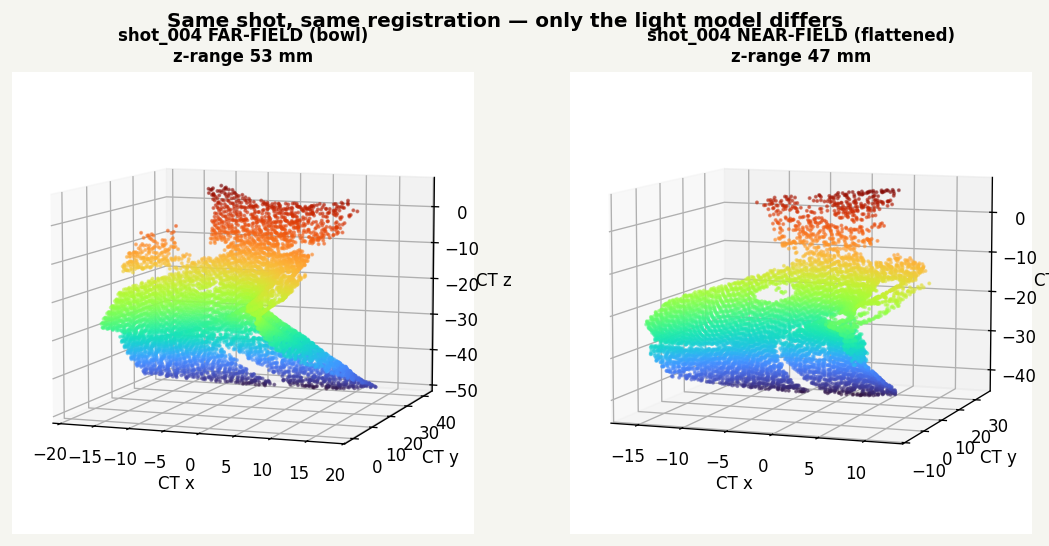
\includegraphics[width=\linewidth]{figures/fig2_bowl.png}
\caption{Level 4, identical registration---only the light model differs. Far-field
(left) integrates a bowl; near-field (right) flattens it.}
\label{fig:bowl}
\end{figure}

\begin{figure}[h]\centering
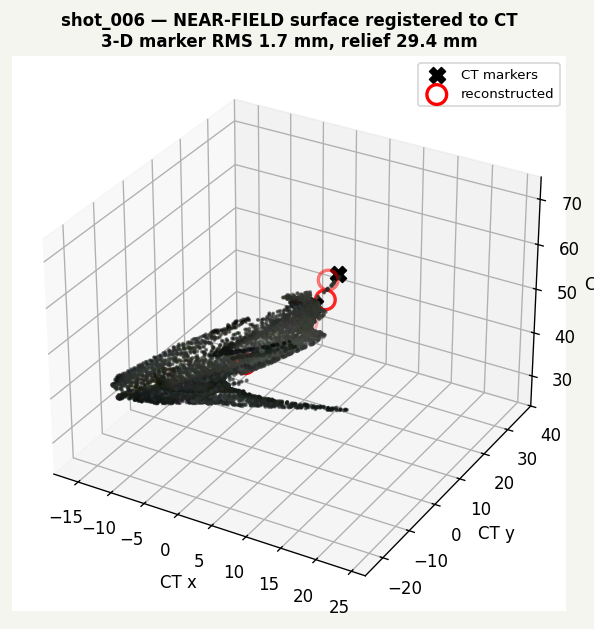
\includegraphics[width=0.72\linewidth]{figures/fig3_shot6.png}
\caption{Level 6 near-field surface registered into CT coordinates; reconstructed
fiducials (open) on CT ground truth (crosses). 3-D FRE \SI{1.7}{\mm}
(far-field \SI{6.6}{\mm}).}
\label{fig:shot6}
\end{figure}

\begin{figure}[h]\centering
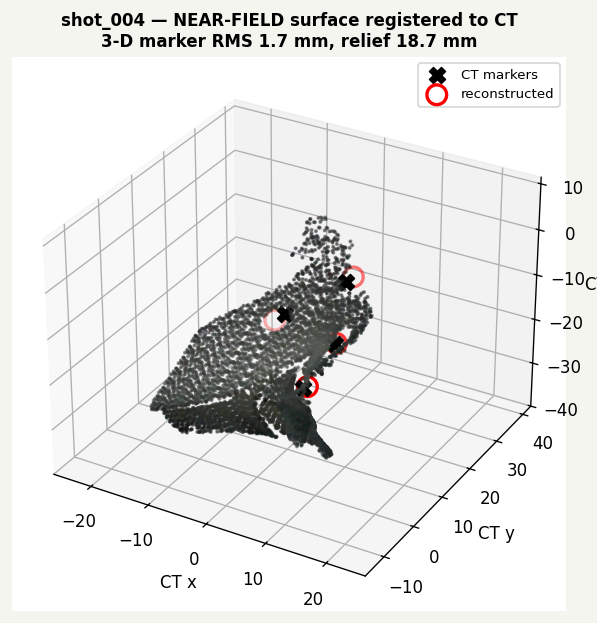
\includegraphics[width=0.72\linewidth]{figures/fig4_shot4.png}
\caption{Level 4 near-field surface registered to CT; 3-D FRE \SI{1.7}{\mm}.}
\label{fig:shot4}
\end{figure}

\subsection{Inverse-square baseline}
A brightness-to-range baseline ($r\propto1/\sqrt{I}$) with identical CT anchoring
failed: \SIrange{7.8}{9.6}{\mm} FRE, dense relief inflating to \SIrange{150}{559}{\mm}
(true CT range \SIrange{17}{26}{\mm}), and a physically inverted depth slope. The
cause is intrinsic---inverse-square assumes constant albedo, so dark bone reads as
``far''---quantifying why the normal-based solve is necessary.

\subsection{Failure modes}
All five levels were imaged at a similar working distance
(\SIrange{51}{60}{\mm}, Table above), so the two failures are not distance-driven.
Level~7 has only three fiducials, leaving the PnP pose under-constrained (P3P admits
up to four solutions). Level~8 has the \emph{best} marker geometry yet the
near-field iteration diverged and the confidence mask collapsed, while the far-field
solve on the same data remained stable (\SI{5.66}{\mm}); this is an unresolved solver
robustness issue, reported rather than omitted. Because working distance was
effectively fixed here, its effect on accuracy could not be characterised; a
controlled distance sweep is future work.

\section{Discussion}
\begin{table}[h]\centering
\caption{Accuracy in context.}
\begin{tabular}{lcc}
\toprule
Method / study & Accuracy & Notes\\
\midrule
\textbf{This work (near-field, 4--6)} & \textbf{\SIrange{1.2}{1.7}{\mm}} & 4 fiducials/level\\
Surface-based spine reg.~\cite{spine} & $\approx$\SI{0.96}{\mm} & 20 points, clinical\\
In-vivo endoscopic PS~\cite{colon} & $<$\SI{3}{\mm} & colon, depth error\\
Near-field light calib.~\cite{aocalib} & $<$\SI{2.7}{\mm} & light position\\
\bottomrule
\end{tabular}
\end{table}

Our millimetre accuracy sits between clinical surface registration and reported
in-vivo endoscopic photometric stereo, with fewer fiducials and a harder near-coaxial
geometry, and---unlike appearance-oriented neural methods---yields a directly
CT-registered metric surface. The contribution is that on a near-coaxial endoscopic
rig the far-field approximation injects a systematic shape error a global scale/offset
cannot remove, and a per-pixel point-source model removes it while preserving
albedo-invariance.

\textbf{Limitations.} (1)~\emph{Assumed LED positions} bound the residual bowl; a
mirror-sphere/matte-target calibration~\cite{queau,aocalib} is the next step,
expected to move levels~6--8 toward \SI{1}{\mm}. (2)~Near-coaxial low SNR compresses
recovered relief. (3)~Reliable only to $\approx$\SI{55}{\mm}. (4)~Three fiducials
under-constrain pose (level~7); specular markers are inpainted, leaving small holes.
(5)~Bench validation on one instrumented specimen; wet in-vivo fields are future work.

\textbf{Clinical relevance.} Per-vertebra registration matches spine navigation
practice; the combined multi-level result is a bench consistency check. A calibrated
CT-registered optical surface from the existing scope could reduce reliance on
intraoperative radiation for re-registration.

\section{Conclusion}
A near-coaxial monocular endoscope, driven by four-LED near-field photometric stereo
and anchored to CT through dual-modality fiducials, reconstructs the exposed spinal
surface to \SIrange{1.2}{1.7}{\mm} per vertebra on well-conditioned levels
---competitive with clinical surface registration and better than reported
in-vivo endoscopic photometric stereo, without added radiation or tracking hardware.
The far-field bowl is removed; the inverse-square shortcut is shown inapplicable to
textured bone; and the dominant residual is localised to assumed LED positions,
defining the next experiment.

\begin{thebibliography}{99}\small
\bibitem{woodham} R.~J. Woodham, ``Photometric method for determining surface
orientation from multiple images,'' \emph{Opt. Eng.}, 19(1), 1980.
\bibitem{fc} R.~T. Frankot, R.~Chellappa, ``A method for enforcing integrability in
shape from shading,'' \emph{IEEE TPAMI}, 10(4), 1988.
\bibitem{queau} Y.~Qu\'eau et al., ``LED-based photometric stereo: modeling,
calibration and numerical solution,'' \emph{JMIV}, 2018. arXiv:1707.01018.
\bibitem{aocalib} ``Robust point light source calibration for near-field
photometric stereo,'' \emph{Applied Optics}, 62(36):9512, 2023.
\bibitem{luces} ``LUCES-MV: multi-view near-field point-light photometric stereo,''
arXiv:2412.16737, 2024.
\bibitem{colon} ``Photometric single-view dense 3D reconstruction in endoscopy,''
arXiv:2204.09083, 2022.
\bibitem{diff2dgs} ``Diff2DGS: reliable reconstruction of occluded surgical scenes,''
arXiv:2602.18314, 2026.
\bibitem{spine} ``Surface-based registration accuracy of CT-based image-guided spine
surgery,'' PubMed 15526221.
\bibitem{fitzpatrick} J.~M. Fitzpatrick, J.~B. West, C.~R. Maurer, ``Predicting error
in rigid-body point-based registration,'' \emph{IEEE TMI}, 17(5), 1998.
\end{thebibliography}

\end{document}
